\pagestyle{empty}
\cleardoublepage
\pagestyle{fancy}

\chapter{Implementação}\label{cap5}

%\section{Introdução}\label{cap5:intro}


\subsection{StarPU}

A aplicação foi feita na linguagem C, com o \emph{framework} StarPU~\citep{starpu}. StarPU  como brevemente citada no capitulo 2, é uma ferramenta para programação paralela que suporta arquiteturas híbridas como CPUs multicore e aceleradores.  StarPU propõe 
uma abordagem de tarefas independentes baseada na arquitetura, para agilizar e facilitar o desenvolvimento de aplicações.

Para a implementação do algoritmo de balanceamento de carga, o StarPU apresenta uma variedade de ferramentas para a implementação da própria política de escalonamento. A principal estrutura utilizada para a implementação da política de escalonamento é a chamada "starpu\_sched\_policy", que é uma estrutura que contém métodos que implementam políticas de escalonamento. A forma de implementação da política de escalonamento consistiu em modificar as estruturas de dados pertencentes ao StarPU, simplificando e adicionando recursos. 

A transferencia de dados consistiu em encapsular dentro de uma tarefa, os dados a serem processados por cada processador. Como utilizamos o conceito de decomposição de domínio, ou seja, os dados são independentes, as tarefas apresentam mesmo grau de prioridade. Assim foi possível utilizar a estrutura do StarPU, que é tem a execução baseada em grafos de tarefas, em um problema de decomposição de domínio. 

Para avaliar o nosso algoritmo de balanceamento de carga, nós modificamos o algoritmo de escalonamento padrão do StarPU. A modificação do algoritmo de balanceamento de carga é feito  alterando a variável STARPU\_SCHED e classes internas do StarPU. O \emph{framework} StarPU tem uma API que permite modificar as políticas de escalonamento. Existem estruturas de dados e funções que aceleram o processo de desenvolvimento. Por exemplo, a função "double starpu\_timing\_now (void)" que retorna a data atual em micro segundos, o que torna mais fácil para a determinação de medidas de tempo de execução. 


\subsection{Multiplicação de Matrizes}

A multiplicação de matrizes ou produto de matrizes é um problema clássico e foi escolhido por ter várias aplicações nos campos da engenharia e ciência, sendo de fácil comparação com os trabalhos da área. De forma visual a multiplicação de matrizes consiste em multiplicar as linhas de uma matriz pelas colunas da segunda matriz e somar, como na figura \ref{matrizes}.

\begin{figure}[htb]
	\begin{center}
	\centering
			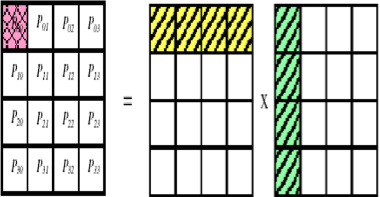
\includegraphics[scale=0.6]{matrizes.png}
	\label{fig: matrizes}
	\caption{Multiplicação de Matrizes}
	\end{center}
\end{figure}

Suponha que existem as matrizes A de N linhas por P colunas e B de P linhas e M colunas o resultado é uma matriz C de N por M colunas. De forma matemática a multiplicação pode ser definida como:

\begin{equation} C_{ij} = \sum_{k=1}^{n_p} A_{ik}B{kj}
 \label{eq:black}
\end{equation}

A paralelização do código se dá dividindo partes das matrizes A e B entre os processadores, seguindo um padrão mestre-escravo. (1) O processo mestre envia trechos da matriz A, e certos número de linhas da matriz.
(2) Cada processo escravo recebe uma matriz de todo o trabalho e recebe um determinado número de linhas da outra matriz. Os nós computam as linhas da matriz de resultado para o número de linhas que recebeu e envia de volta para o mestre. 
(3) O processo mestre agora recolhe as linhas da matriz de resultados do escravo, juntamente com o seu deslocamento na matriz resultado. 

O algoritmo utiliza um processo principal e uma série de tarefas escravas independentes. A implementação varia dependendo do modelo GPU, CPU, mas o conceito de divisão dos dados é o mesmo. Não foi utilizado nenhuma otimização no código da versão em GPU, tal como a utilização de um algoritmo mais eficaz para a multiplicação de matrizes, as únicas otimizações se referem a melhor utilização do hardware, como por exemplo o uso de memória compartilhada, e a divisão dos dados entre os blocos de threads, de forma a utilizar todas as threads de cada bloco, a divisão depende do modelo de placa, mas são configurações simples de serem feitas e não afetam a usabilidade do algoritmo de balanceamento de carga. 

\subsection{Blackscholes}

O modelo Blackcholes é um modelo matemático de mercado financeiro contendo certo instrumentos de investimento. Do modelo, o que pode ser deduzido é a fórmula Blackscholes, que nos fornece a estimativa teórica dos preços de opções no estilo europeu. Em finanças, uma opção é um contrato que dá ao comprador (o proprietário) o direito, mas não a obrigação, de comprar ou vender um ativo ou instrumento subjacente, a um preço determinado antes de uma data especificada. O vendedor tem a obrigação de cumprir a operação, que é a de vender ou comprar. Uma opção que transmite ao titular o direito de comprar algo a um preço específico é referida como uma chamada; uma opção que transmite o direito do proprietário para vender algo a um preço específico é referida como uma opção de venda. Ambos são comumente negociadas, mas para maior clareza, a opção de compra é mais freqüentemente discutidos. A fórmula levou a um "boom" na negociação de opções e legitimou cientificamente as atividades da Chicago Board Options Exchange e outros mercados de opções ao redor do mundo. Muitos testes empíricos têm demonstrado que o preço de Black-Scholes é "bastante próximo" aos preços observados, embora haja discrepâncias bem conhecidas. 


O modelo de Blackscholes foi publicado por Fischer Black e Myron Scholes em 1973, em um artigo entitulado \emph{"The Pricing of Options and Corporate Liabilities"}, publicado no \emph{Journal of Political Economy}. Eles derivaram uma equação diferencial parcial, agora chamada de equação de Black-Scholes, que estima o preço da opção ao longo do tempo. 

Robert C. Merton foi o primeiro a publicar um artigo ampliando a compreensão matemática do modelo de precificação de opções, e cunhou o termo "Black-Scholes de precificação de opções". Merton e Scholes receberam o Prêmio Nobel de Economia em 1997 (O Prêmio Sveriges Riksbank em Ciências Econômicas em Memória de Alfred Nobel) por seu trabalho. Embora inelegível para o prêmio por causa de sua morte, em 1995, Black foi mencionado como um contribuinte pela Academia Sueca. 

Pressupostos do modelo foram relaxadas e generalizados em muitas vertentes, levando a uma infinidade de modelos que são atualmente utilizados em precificação de derivativos e gestão de riscos. É os insights do modelo, como exemplificado na fórmula Black-Scholes, que são frequentemente utilizados pelos participantes do mercado, como distinguir entre os preços reais. A equação de Black-Scholes, uma equação diferencial parcial que governa o preço da opção, também é importante, pois permite se colocar preços quando uma fórmula explícita não é possível. 

A fórmula Black-Scholes tem apenas um parâmetro que não pode ser observada no mercado: a volatilidade futura média do ativo. Uma vez que a fórmula é o aumento neste parâmetro, ela pode ser invertida de modo a produzir uma superfície de volatilidade que é então utilizado para calibrar outros modelos. A equação do Blackscholes é a seguinte:

\begin{equation} \frac {\delta V}{\delta t} + \frac{1}{2} \sigma^2 S^2 \frac{\delta^2 V}{\delta S^2} + rS \frac{\delta V}{\delta S} - rV = 0
 \label{eq:black}
\end{equation}

onde V é o preço da opção em função do preço das ações S e t é o tempo, r é a taxa de juros livre de risco, e $\sigma$ é a volatilidade das ações.

O principal problema da implementação em CUDA da fórmula Blackscholes é escolher o melhor \emph{layout} de armazenamento de dados. A implementação do \emph{kernel} utilizada foi a fornecida pela API do Cuda. A implementação consiste em atribuir a cada thread um 
índice específico dos dados de entrada. A divisão dos dados na StarPU basicamente, é dividir as opções entre os processadores de forma direta. 


\subsection{Explicação dos algoritmos}

Três outros algoritmos foram implementados para comparação: o guloso (StarPU), o estático e o
HDSS. O guloso consistiu em dividir o conjunto de entrada em pedaços e atribuir 
cada pedaço da entrada a qualquer processador ocioso, sem qualquer atribuição de prioridade. O estático~\citep{raphael}, mede as velocidades de processamento antes da execução e  atribui um conjunto  de blocos estático para cada processador, no início da execução, com os
tamanhos do bloco proporcional à velocidade do processador. Por fim, o HDSS~\citep{HDSS}  
utiliza a estimativa dos mínimos quadrados para estimar a curva logarítmica e divide em duas fases: fase de adaptação e fase de conclusão. 

\subsubsection{HDSS - Heterogeneous Dynamic Self-Scheduler}

O algoritmo HDSS~\citep{hdss} determina o tamanho do bloco por processador usando uma abordagem em duas fases. A fase inicial, chamada de fase de adaptação, é responsável por encontrar os pesos computacionais que refletem as velocidades relativas de cada processador. Esta fase processa uma quantidade relativamente pequena de dados, cujo limite superior é definido como uma percentagem fixa do total de dados. A fase final, chamada fase de conclusão, processa o restante dos dados, usando os pesos calculados na fase adaptativa. Esta fase começa com os maiores blocos possíveis para otimizar o tempo de execução. O tamanho do bloco diminui progressivamente à medida que a computação trabalha no sentido final para que todas as unidades de execução completem, quase ao mesmo tempo.  O conceito do algoritmo é em um primeiro momento encontrar pesos para serem usados posteriormente na fase de conclusão, esses pesos darão a forma com que os dados devem ser divididos entre os processadores.  Os pesos são determinados com base em ajustes em gráficos logaritmicos de processamento. As principais diferenças do algoritmo proposto o nosso modelo não se restringe a curvas logarítimocas, além de se ajustar até o fim da execução.



\subsection{IPOPT}

A biblioteca utilizada para resolver o sistema de equações é a IPOPT~\citep{point}. IPOPT \emph{(Interior Point Optimizer)} é um pacote de software de código aberto para otimização não-linear em grande escala. Ele pode ser utilizado para resolver problemas de programação lineares gerais, da forma:

\begin{eqnarray}
\displaystyle \min_{x\in\mathbb{R}^n} 
	\displaystyle f(x) \\
	s.a.\displaystyle \;  \nonumber 
	 	\displaystyle g^L \leq g(x) \leq g^U  \nonumber \\	
 	 	\displaystyle x^L \leq x \leq x^U, \nonumber 
\end{eqnarray}

onde $x$, $\in$, $\Re ^ n$ são as variáveis de otimização, $f : R^n$ em $R$ é a função objetivo, e $g: R^n$ em $R^M$ são as restrições não lineares. A função $f(x)$ e $g(x)$ podem ser linear ou não linear.  

Para resolver um problema de otimização precisa-se criar um IpoptProblem com a função CreateIpoptProblem, que posteriormente precisa ser passado para a função IpoptSolve. O IpoptProblem criado por CreateIpoptProblem contem as dimensões do problema, as variáveis e os limites das restrições. A execução da resolução torna-se apenas um processo de correta montagem do problema a ser tratado. O algoritmo leva certo tempo para resolver o problema que é na ordem dos milissegundos. 


